\clearpage

\part{Testing} % (fold)
\label{prt:testing_}
This initial part of the documentation features the analysis that was performed on the business. It includes the business' background, as well as an in-depth investigation on their current system, featuring document inspections, interviews, and observations. Also included is a problem definition, wherein the broad aims of the project are outlined; this definition also makes reference to the limitations of the solution. Finally, detailed objectives are clearly laid out, providing an overview of exactly what the solution should achieve.

% Import test_strategy
\section{Test Strategy}
This test strategy details the overall strategy that will be used to test the application.


% Import test_plan
\section{Test Plan}
This section contains detailed test plans for each part of the system. Each individual test plan includes the part of the system that is being tested, the steps that should be performed, the data to be entered and the expected outcome.

% \subsection{Login Screen Testing} % (fold)
\label{sub:login_screen_testing}
This subsection states how to test that the system themes itself correctly for each house.
% subsection login_screen_testing (end)

\subsubsection{Display Acton Colours} % (fold)
\label{ssub:display_acton_colours}
\begin{enumerate}[leftmargin=*]
\item Select ``Acton'' in the house box.\\\\
\textit{Expected result}: Interface should turn blue.
\end{enumerate}
% subsubsection display_acton_colours (end)

\subsubsection{Display Baxter Colours} % (fold)
\label{ssub:display_baxter_colours}
\begin{enumerate}[leftmargin=*]
\item Select ``Baxter'' in the house box.\\\\
\textit{Expected result}: Interface should turn orange.
\end{enumerate}
% subsubsection display_baxter_colours (end)

\subsubsection{Display Clive Colours} % (fold)
\label{ssub:display_clive_colours}
\begin{enumerate}[leftmargin=*]
\item Select ``Clive'' in the house box.\\\\
\textit{Expected result}: Interface should turn green.
\end{enumerate}
% subsubsection display_clive_colours (end)

\subsubsection{Display Darwin Colours} % (fold)
\label{ssub:display_darwin_colours}
\begin{enumerate}[leftmargin=*]
\item Select ``Darwin'' in the house box.\\\\
\textit{Expected result}: Interface should turn purple.
\end{enumerate}
% subsubsection display_darwin_colours (end)

\subsubsection{Display Houseman Colours} % (fold)
\label{ssub:display_houseman_colours}
\begin{enumerate}[leftmargin=*]
\item Select ``Houseman'' in the house box.\\\\
\textit{Expected result}: Interface should turn red.
\end{enumerate}
% subsubsection display_houseman_colours (end)

\subsubsection{Display Webb Colours} % (fold)
\label{ssub:display_webb_colours}
\begin{enumerate}[leftmargin=*]
\item Select ``Webb'' in the house box.\\\\
\textit{Expected result}: Interface should turn yellow.
\end{enumerate}
% subsubsection display_webb_colours (end)

\subsection{Navigation Tests}
This section tests that the navigation in the application works correctly; i.e. that each main link leads to the correct part of the application.

\begin{table}[]
\centering
\begin{tabular}{|l|l|l|l|}
\hline
\multicolumn{1}{|c|}{\textbf{Link}} & \multicolumn{1}{c|}{\textbf{Expected result}} & \multicolumn{1}{c|}{\textbf{Actual result}} & \multicolumn{1}{c|}{\textbf{Teacher signature}} \\ \hline
/                                   & Login screen.                                 & As expected.                                &                                                 \\ \hline
/create                             & Navigate to quiz creator.                     & As expected.                                &                                                 \\ \hline
/play                               & Navigate to quiz player.                      & As expected.                                &                                                 \\ \hline
\end{tabular}
\caption{Application navigation}
\label{application-navigation}
\end{table}

\subsection{Login Test Runs}
This subsection contains the test runs for the login screen, using as a reference the login screen test plan available at 13.1.

\subsubsection{Load Quizzes}
This test ensures that a list of all available quizzes can be searched for and found on the login screen, ready to either edit or delete.

\begin{figure}[!htbp]
\centering
\begin{subfigure}{0.5\textwidth}
  \centering
  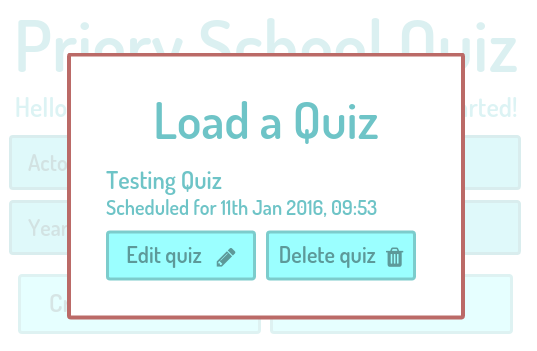
\includegraphics[width=0.95\linewidth]{testing/load_quiz/single_quiz}
  \caption{Single quiz (typical)}
  \label{fig:sub1}
\end{subfigure}%
\begin{subfigure}{0.5\textwidth}
  \centering
  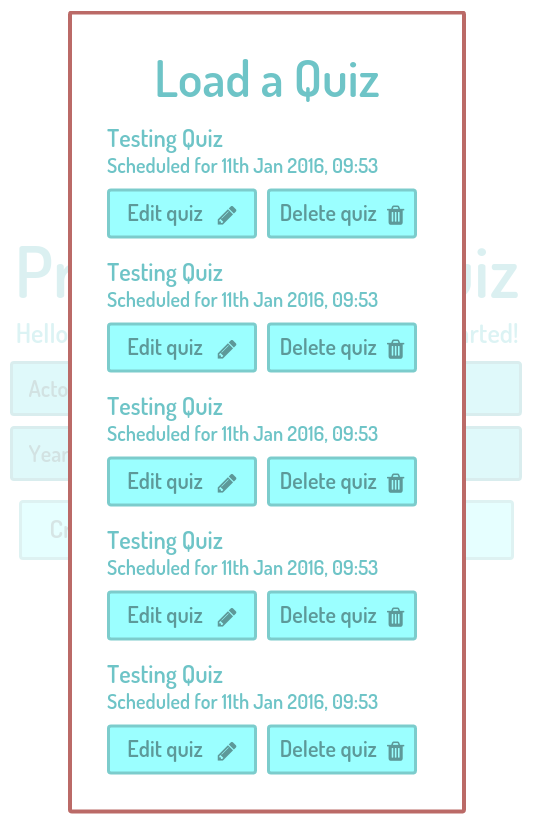
\includegraphics[width=0.95\linewidth]{testing/load_quiz/multiple_quizzes}
  \caption{Five quizzes (extreme)}
  \label{fig:sub2}
\end{subfigure}
\begin{subfigure}{0.5\textwidth}
  \centering
  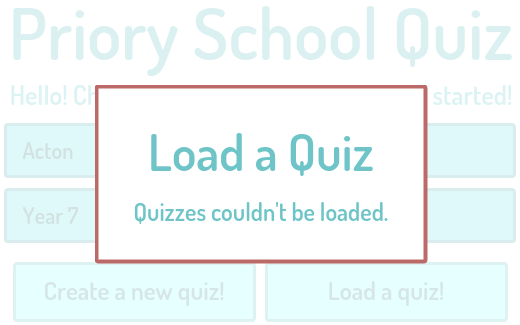
\includegraphics[width=0.95\linewidth]{testing/load_quiz/offline}
  \caption{No connection (erroneous)}
  \label{fig:sub2}
\end{subfigure}
\begin{subfigure}{0.5\textwidth}
  \centering
  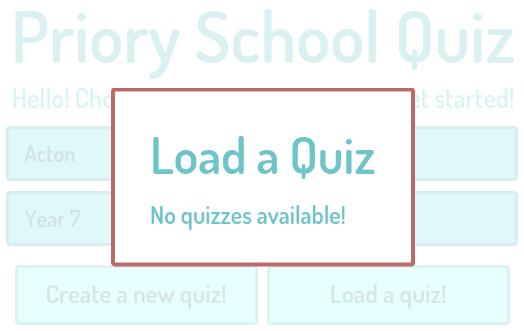
\includegraphics[width=0.95\linewidth]{testing/load_quiz/no_quizzes}
  \caption{No quizzes (null)}
  \label{fig:sub2}
\end{subfigure}
\caption{The load quiz dialog.}
\label{fig:test}
\end{figure}
As can be seen, all the tests have worked successfully: when there is only a single quiz in the database, only a single quiz is shown; when there are five, all of these are listed; when there is no connection, and the system is unable to perform an API call, the correct error message is shown; and when there are simply no quizzes available, this too is properly relayed to the user. \textit{Success.}

\subsection{Create Quiz Test Runs} % (fold)
\label{sub:create_quiz_test}
This section contains the test runs performed on the quiz creator.


\subsubsection{Add Question} % (fold)
\label{ssub:add_question}
This ensures that the user is able to succesfully add a new question to the current quiz when the add question button is pressed.
\begin{figure}[!htbp]
\centering
\begin{subfigure}{0.5\textwidth}
  \centering
  \includegraphics[width=0.95\linewidth]{testing/create_quiz/add_question/before}
  \caption{Before}
  \label{fig:sub1}
\end{subfigure}%
\begin{subfigure}{0.5\textwidth}
  \centering
  \includegraphics[width=0.95\linewidth]{testing/create_quiz/add_question/after}
  \caption{After}
  \label{fig:sub2}
\end{subfigure}
\caption{Adding a question to the quiz.}
\label{fig:test}
\end{figure}
\\As the two pictures indicate, after pressing the add question button, a new question was added to the system, and this was reflectd in the label unde the question title. \textit{Success.}
% subsubsection add_question (end)

\clearpage

\subsubsection{Edit Question} % (fold)
\label{ssub:edit_question}
This ensures that the user is able to succesfully edit a question in the current quiz.
\begin{figure}[!htbp]
\begin{subfigure}{0.5\textwidth}
  \centering
  \includegraphics[width=0.95\linewidth]{testing/create_quiz/edit_question/during}
  \caption{During}
  \label{fig:sub2}
\end{subfigure}
\begin{subfigure}{0.5\textwidth}
  \centering
  \includegraphics[width=0.95\linewidth]{testing/create_quiz/edit_question/after}
  \caption{After}
  \label{fig:sub3}
\end{subfigure}
\caption{Editing a question to the quiz.}
\label{fig:test}
\end{figure}
% subsubsection edit_question (end)


\subsubsection{Delete Question} % (fold)
\label{ssub:delete_question}
This ensures that the user is able to succesfully delete their questions from the current quiz.
\\\\\textit{\textbf{Note:} In order to prove that the question has actually been deleted, the screenshot captures the developer tools used in the creation of the application; an action showing that the question has been deleted is clearly visible.}
\begin{figure}[!htbp]
\centering
\begin{subfigure}{0.5\textwidth}
  \centering
  \includegraphics[width=0.95\linewidth]{testing/create_quiz/delete_question/before}
  \caption{Before}
  \label{fig:sub1}
\end{subfigure}%
\begin{subfigure}{0.5\textwidth}
  \centering
  \includegraphics[width=0.95\linewidth]{testing/create_quiz/delete_question/after}
  \caption{After}
  \label{fig:sub2}
\end{subfigure}
\caption{Delete a question in the quiz.}
\label{fig:test}
\end{figure}
\\The second screenshot shows that a delete question action was passed to the quiz reducer, resulting in the question being successfully deleted; this is also reflected in the labels. \textit{Success.}
% subsubsection delete_question (end)


\subsubsection{Add Category} % (fold)
\label{ssub:add_category}
This ensures that the user is able to succesfully add a custom category to the current quiz.
\begin{figure}[!htbp]
\centering
\begin{subfigure}{0.5\textwidth}
  \centering
  \includegraphics[width=0.95\linewidth]{testing/create_quiz/add_category/during}
  \caption{During}
  \label{fig:sub1}
\end{subfigure}%
\begin{subfigure}{0.5\textwidth}
  \centering
  \includegraphics[width=0.95\linewidth]{testing/create_quiz/add_category/after}
  \caption{After}
  \label{fig:sub2}
\end{subfigure}
\caption{Adding a category to the quiz.}
\label{fig:test}
\end{figure}
As expected, a dialog to enter a category name is shown when the add category button is pressed, and the new category is added successfully. \textit{Success.}
% subsubsection add_category (end)


\subsubsection{Delete Category} % (fold)
\label{ssub:add_category}
This ensures that the user is able to succesfully delete their custom categories in the current quiz.
\begin{figure}[!htbp]
\centering
\begin{subfigure}{0.5\textwidth}
  \centering
  \includegraphics[width=0.95\linewidth]{testing/create_quiz/delete_category/before}
  \caption{Before}
  \label{fig:sub1}
\end{subfigure}%
\begin{subfigure}{0.5\textwidth}
  \centering
  \includegraphics[width=0.95\linewidth]{testing/create_quiz/delete_category/after}
  \caption{After}
  \label{fig:sub2}
\end{subfigure}
\caption{Deleting a category from the quiz.}
\label{fig:test}
\end{figure}
As expected, a dialog to enter a category name is shown when the add category button is pressed, and the new category is added successfully. \textit{Success.}
% subsubsection add_category (end)


\subsubsection{Rename Category} % (fold)
\label{ssub:add_category}
This ensures that the user is able to succesfully rename their custom categories in the current quiz.
\begin{figure}[!htbp]
\centering
\begin{subfigure}{0.5\textwidth}
  \centering
  \includegraphics[width=0.95\linewidth]{testing/create_quiz/rename_category/during}
  \caption{During}
  \label{fig:sub1}
\end{subfigure}%
\begin{subfigure}{0.5\textwidth}
  \centering
  \includegraphics[width=0.95\linewidth]{testing/create_quiz/rename_category/after}
  \caption{After}
  \label{fig:sub2}
\end{subfigure}
\caption{Renaming a category in the quiz.}
\label{fig:test}
\end{figure}
As expected, a dialog to enter the new category name is shown when the rename category button is pressed, and category is renamed successfully. \textit{Success.}
% subsubsection add_category (end)

\subsubsection{Edit Answer} % (fold)
\label{ssub:add_category}
This test ensures that the user is able to edit the body of an answer in the current quiz.
\begin{figure}[!htbp]
\centering
\begin{subfigure}{0.5\textwidth}
  \centering
  \includegraphics[width=0.95\linewidth]{testing/create_quiz/edit_answer/during}
  \caption{During}
  \label{fig:sub1}
\end{subfigure}%
\begin{subfigure}{0.5\textwidth}
  \centering
  \includegraphics[width=0.95\linewidth]{testing/create_quiz/edit_answer/after}
  \caption{After}
  \label{fig:sub2}
\end{subfigure}
\caption{Marking an answer in as correct.}
\label{fig:test}
\end{figure}
\\As expected, the application allowed for the answer body to be edited, and then persisted this change after leaving the edit mode. \textit{Success.}
% subsubsection add_category (end)


\subsubsection{Mark Answer as Correct} % (fold)
\label{ssub:add_category}
This ensures that the user is able to succesfully mark an answer as correct in the current quiz.
\begin{figure}[!htbp]
\centering
\begin{subfigure}{0.5\textwidth}
  \centering
  \includegraphics[width=0.95\linewidth]{testing/create_quiz/change_answer/before}
  \caption{During}
  \label{fig:sub1}
\end{subfigure}%
\begin{subfigure}{0.5\textwidth}
  \centering
  \includegraphics[width=0.95\linewidth]{testing/create_quiz/change_answer/after}
  \caption{After}
  \label{fig:sub2}
\end{subfigure}
\caption{Marking an answer in as correct.}
\label{fig:test}
\end{figure}
\\As expected, the correct mark moved from the third to the first question, meaning that it was marked as correct. \textit{Success.}
% subsubsection add_category (end)


\subsubsection{Save Quiz} % (fold)
\label{ssub:add_category}
This test ensures that the user is able to save their quizzes to the database.
\begin{figure}[!htbp]
\centering
\begin{subfigure}{0.5\textwidth}
  \centering
  \includegraphics[width=0.95\linewidth]{testing/create_quiz/save_quiz/before}
  \caption{During}
  \label{fig:sub1}
\end{subfigure}%
\begin{subfigure}{0.5\textwidth}
  \centering
  \includegraphics[width=0.95\linewidth]{testing/create_quiz/save_quiz/after}
  \caption{After}
  \label{fig:sub2}
\end{subfigure}
\caption{Saving a quiz to the database.}
\label{fig:test}
\end{figure}
\\As expected, the correct mark moved from the third to the first question, meaning that it was marked as correct. \textit{Success.}
% subsubsection add_category (end)

\subsubsection{Move Questions on Time}
This test ensures that the quiz moves to the correct questions at the correct time, using the test quiz specified in the test plan. Due to the difficulty of taking valid screenshots of this process, a table is included below with room for a teacher to sign as confirmation that this functionality is working.

\begin{table}[]
\centering
\begin{tabular}{|l|l|l|}
\hline
\multicolumn{1}{|c|}{\textbf{Expected result}}              & \multicolumn{1}{c|}{\textbf{Works}} & \multicolumn{1}{c|}{\textbf{Signature}} \\ \hline
Displays "Who is the French Premier?" at 0-10 seconds       & Yes                                 &                                         \\ \hline
Displays "Who won the 1960 World Cup?" at 10-20 seconds     & Yes                                 &                                         \\ \hline
Displays "What is the capital of Iceland?" at 20-30 seconds & Yes                                 &                                         \\ \hline
\end{tabular}
\caption{My caption}
\label{my-label}
\end{table}

\\As can be witnessed, the quiz moves to the correct questions at the correct time, meaning that the test has passed. \texit{Success.}

\subsection{Results Test Runs} % (fold)
\label{sub:results_test_runs}
This section tests that the results screen works correctly.

\subsubsection{Connects to State Store} % (fold)
\label{ssub:connects_to_state_store}
This test ensures that the component can connect to the state store.
% subsubsection connects_to_state_store (end)

\subsubsection{Display Correct Results} % (fold)
\label{ssub:display_correct_results}
This test ensures that the results screen shows the correct results.
% subsubsection display_correct_results (end)
% subsection results_test_runs (end)


% Import test_runs
\clearpage
\section{Test Runs}
These are the actual test runs, indicating whether or not a test has successfully completed. For each test, the unit test code is included, followed by a screenshot of the test outcome. If a test is unsuccessful, the changes made to the code will be shown, followed by another screenshot of the test outcome.

\subsection{Login Test Runs}
This subsection contains the test runs for the login screen, using as a reference the login screen test plan available at 13.1.

\subsubsection{Load Quizzes}
This test ensures that a list of all available quizzes can be searched for and found on the login screen, ready to either edit or delete.

\begin{figure}[!htbp]
\centering
\begin{subfigure}{0.5\textwidth}
  \centering
  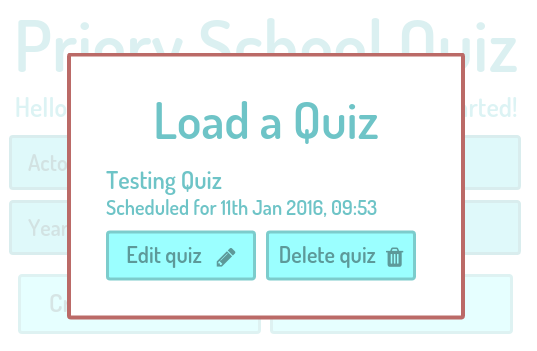
\includegraphics[width=0.95\linewidth]{testing/load_quiz/single_quiz}
  \caption{Single quiz (typical)}
  \label{fig:sub1}
\end{subfigure}%
\begin{subfigure}{0.5\textwidth}
  \centering
  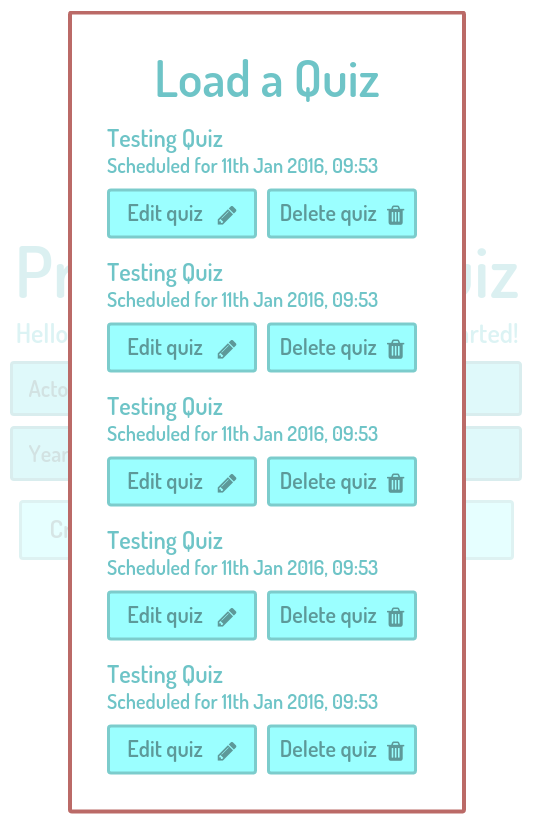
\includegraphics[width=0.95\linewidth]{testing/load_quiz/multiple_quizzes}
  \caption{Five quizzes (extreme)}
  \label{fig:sub2}
\end{subfigure}
\begin{subfigure}{0.5\textwidth}
  \centering
  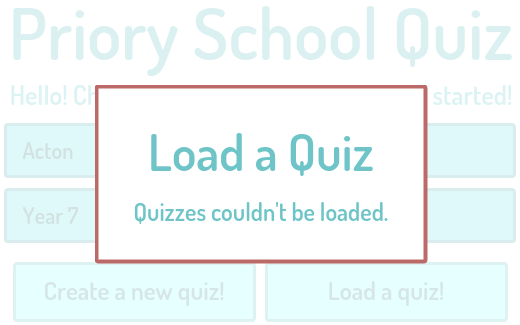
\includegraphics[width=0.95\linewidth]{testing/load_quiz/offline}
  \caption{No connection (erroneous)}
  \label{fig:sub2}
\end{subfigure}
\begin{subfigure}{0.5\textwidth}
  \centering
  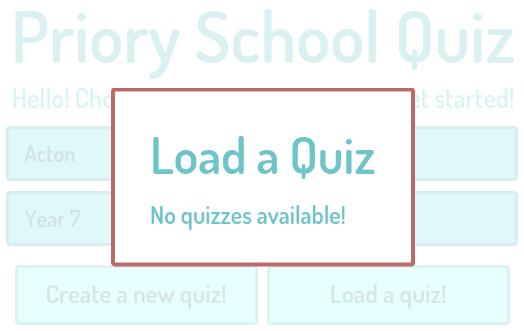
\includegraphics[width=0.95\linewidth]{testing/load_quiz/no_quizzes}
  \caption{No quizzes (null)}
  \label{fig:sub2}
\end{subfigure}
\caption{The load quiz dialog.}
\label{fig:test}
\end{figure}
As can be seen, all the tests have worked successfully: when there is only a single quiz in the database, only a single quiz is shown; when there are five, all of these are listed; when there is no connection, and the system is unable to perform an API call, the correct error message is shown; and when there are simply no quizzes available, this too is properly relayed to the user. \textit{Success.}

\subsection{Create Quiz Test Runs} % (fold)
\label{sub:create_quiz_test}
This section contains the test runs performed on the quiz creator.


\subsubsection{Add Question} % (fold)
\label{ssub:add_question}
This ensures that the user is able to succesfully add a new question to the current quiz when the add question button is pressed.
\begin{figure}[!htbp]
\centering
\begin{subfigure}{0.5\textwidth}
  \centering
  \includegraphics[width=0.95\linewidth]{testing/create_quiz/add_question/before}
  \caption{Before}
  \label{fig:sub1}
\end{subfigure}%
\begin{subfigure}{0.5\textwidth}
  \centering
  \includegraphics[width=0.95\linewidth]{testing/create_quiz/add_question/after}
  \caption{After}
  \label{fig:sub2}
\end{subfigure}
\caption{Adding a question to the quiz.}
\label{fig:test}
\end{figure}
\\As the two pictures indicate, after pressing the add question button, a new question was added to the system, and this was reflectd in the label unde the question title. \textit{Success.}
% subsubsection add_question (end)

\clearpage

\subsubsection{Edit Question} % (fold)
\label{ssub:edit_question}
This ensures that the user is able to succesfully edit a question in the current quiz.
\begin{figure}[!htbp]
\begin{subfigure}{0.5\textwidth}
  \centering
  \includegraphics[width=0.95\linewidth]{testing/create_quiz/edit_question/during}
  \caption{During}
  \label{fig:sub2}
\end{subfigure}
\begin{subfigure}{0.5\textwidth}
  \centering
  \includegraphics[width=0.95\linewidth]{testing/create_quiz/edit_question/after}
  \caption{After}
  \label{fig:sub3}
\end{subfigure}
\caption{Editing a question to the quiz.}
\label{fig:test}
\end{figure}
% subsubsection edit_question (end)


\subsubsection{Delete Question} % (fold)
\label{ssub:delete_question}
This ensures that the user is able to succesfully delete their questions from the current quiz.
\\\\\textit{\textbf{Note:} In order to prove that the question has actually been deleted, the screenshot captures the developer tools used in the creation of the application; an action showing that the question has been deleted is clearly visible.}
\begin{figure}[!htbp]
\centering
\begin{subfigure}{0.5\textwidth}
  \centering
  \includegraphics[width=0.95\linewidth]{testing/create_quiz/delete_question/before}
  \caption{Before}
  \label{fig:sub1}
\end{subfigure}%
\begin{subfigure}{0.5\textwidth}
  \centering
  \includegraphics[width=0.95\linewidth]{testing/create_quiz/delete_question/after}
  \caption{After}
  \label{fig:sub2}
\end{subfigure}
\caption{Delete a question in the quiz.}
\label{fig:test}
\end{figure}
\\The second screenshot shows that a delete question action was passed to the quiz reducer, resulting in the question being successfully deleted; this is also reflected in the labels. \textit{Success.}
% subsubsection delete_question (end)


\subsubsection{Add Category} % (fold)
\label{ssub:add_category}
This ensures that the user is able to succesfully add a custom category to the current quiz.
\begin{figure}[!htbp]
\centering
\begin{subfigure}{0.5\textwidth}
  \centering
  \includegraphics[width=0.95\linewidth]{testing/create_quiz/add_category/during}
  \caption{During}
  \label{fig:sub1}
\end{subfigure}%
\begin{subfigure}{0.5\textwidth}
  \centering
  \includegraphics[width=0.95\linewidth]{testing/create_quiz/add_category/after}
  \caption{After}
  \label{fig:sub2}
\end{subfigure}
\caption{Adding a category to the quiz.}
\label{fig:test}
\end{figure}
As expected, a dialog to enter a category name is shown when the add category button is pressed, and the new category is added successfully. \textit{Success.}
% subsubsection add_category (end)


\subsubsection{Delete Category} % (fold)
\label{ssub:add_category}
This ensures that the user is able to succesfully delete their custom categories in the current quiz.
\begin{figure}[!htbp]
\centering
\begin{subfigure}{0.5\textwidth}
  \centering
  \includegraphics[width=0.95\linewidth]{testing/create_quiz/delete_category/before}
  \caption{Before}
  \label{fig:sub1}
\end{subfigure}%
\begin{subfigure}{0.5\textwidth}
  \centering
  \includegraphics[width=0.95\linewidth]{testing/create_quiz/delete_category/after}
  \caption{After}
  \label{fig:sub2}
\end{subfigure}
\caption{Deleting a category from the quiz.}
\label{fig:test}
\end{figure}
As expected, a dialog to enter a category name is shown when the add category button is pressed, and the new category is added successfully. \textit{Success.}
% subsubsection add_category (end)


\subsubsection{Rename Category} % (fold)
\label{ssub:add_category}
This ensures that the user is able to succesfully rename their custom categories in the current quiz.
\begin{figure}[!htbp]
\centering
\begin{subfigure}{0.5\textwidth}
  \centering
  \includegraphics[width=0.95\linewidth]{testing/create_quiz/rename_category/during}
  \caption{During}
  \label{fig:sub1}
\end{subfigure}%
\begin{subfigure}{0.5\textwidth}
  \centering
  \includegraphics[width=0.95\linewidth]{testing/create_quiz/rename_category/after}
  \caption{After}
  \label{fig:sub2}
\end{subfigure}
\caption{Renaming a category in the quiz.}
\label{fig:test}
\end{figure}
As expected, a dialog to enter the new category name is shown when the rename category button is pressed, and category is renamed successfully. \textit{Success.}
% subsubsection add_category (end)

\subsubsection{Edit Answer} % (fold)
\label{ssub:add_category}
This test ensures that the user is able to edit the body of an answer in the current quiz.
\begin{figure}[!htbp]
\centering
\begin{subfigure}{0.5\textwidth}
  \centering
  \includegraphics[width=0.95\linewidth]{testing/create_quiz/edit_answer/during}
  \caption{During}
  \label{fig:sub1}
\end{subfigure}%
\begin{subfigure}{0.5\textwidth}
  \centering
  \includegraphics[width=0.95\linewidth]{testing/create_quiz/edit_answer/after}
  \caption{After}
  \label{fig:sub2}
\end{subfigure}
\caption{Marking an answer in as correct.}
\label{fig:test}
\end{figure}
\\As expected, the application allowed for the answer body to be edited, and then persisted this change after leaving the edit mode. \textit{Success.}
% subsubsection add_category (end)


\subsubsection{Mark Answer as Correct} % (fold)
\label{ssub:add_category}
This ensures that the user is able to succesfully mark an answer as correct in the current quiz.
\begin{figure}[!htbp]
\centering
\begin{subfigure}{0.5\textwidth}
  \centering
  \includegraphics[width=0.95\linewidth]{testing/create_quiz/change_answer/before}
  \caption{During}
  \label{fig:sub1}
\end{subfigure}%
\begin{subfigure}{0.5\textwidth}
  \centering
  \includegraphics[width=0.95\linewidth]{testing/create_quiz/change_answer/after}
  \caption{After}
  \label{fig:sub2}
\end{subfigure}
\caption{Marking an answer in as correct.}
\label{fig:test}
\end{figure}
\\As expected, the correct mark moved from the third to the first question, meaning that it was marked as correct. \textit{Success.}
% subsubsection add_category (end)


\subsubsection{Save Quiz} % (fold)
\label{ssub:add_category}
This test ensures that the user is able to save their quizzes to the database.
\begin{figure}[!htbp]
\centering
\begin{subfigure}{0.5\textwidth}
  \centering
  \includegraphics[width=0.95\linewidth]{testing/create_quiz/save_quiz/before}
  \caption{During}
  \label{fig:sub1}
\end{subfigure}%
\begin{subfigure}{0.5\textwidth}
  \centering
  \includegraphics[width=0.95\linewidth]{testing/create_quiz/save_quiz/after}
  \caption{After}
  \label{fig:sub2}
\end{subfigure}
\caption{Saving a quiz to the database.}
\label{fig:test}
\end{figure}
\\As expected, the correct mark moved from the third to the first question, meaning that it was marked as correct. \textit{Success.}
% subsubsection add_category (end)

\subsubsection{Move Questions on Time}
This test ensures that the quiz moves to the correct questions at the correct time, using the test quiz specified in the test plan. Due to the difficulty of taking valid screenshots of this process, a table is included below with room for a teacher to sign as confirmation that this functionality is working.

\begin{table}[]
\centering
\begin{tabular}{|l|l|l|}
\hline
\multicolumn{1}{|c|}{\textbf{Expected result}}              & \multicolumn{1}{c|}{\textbf{Works}} & \multicolumn{1}{c|}{\textbf{Signature}} \\ \hline
Displays "Who is the French Premier?" at 0-10 seconds       & Yes                                 &                                         \\ \hline
Displays "Who won the 1960 World Cup?" at 10-20 seconds     & Yes                                 &                                         \\ \hline
Displays "What is the capital of Iceland?" at 20-30 seconds & Yes                                 &                                         \\ \hline
\end{tabular}
\caption{My caption}
\label{my-label}
\end{table}

\\As can be witnessed, the quiz moves to the correct questions at the correct time, meaning that the test has passed. \texit{Success.}

\subsection{Login Screen Testing} % (fold)
\label{sub:login_screen_testing}
This subsection states how to test that the system themes itself correctly for each house.
% subsection login_screen_testing (end)

\subsubsection{Display Acton Colours} % (fold)
\label{ssub:display_acton_colours}
\begin{enumerate}[leftmargin=*]
\item Select ``Acton'' in the house box.\\\\
\textit{Expected result}: Interface should turn blue.
\end{enumerate}
% subsubsection display_acton_colours (end)

\subsubsection{Display Baxter Colours} % (fold)
\label{ssub:display_baxter_colours}
\begin{enumerate}[leftmargin=*]
\item Select ``Baxter'' in the house box.\\\\
\textit{Expected result}: Interface should turn orange.
\end{enumerate}
% subsubsection display_baxter_colours (end)

\subsubsection{Display Clive Colours} % (fold)
\label{ssub:display_clive_colours}
\begin{enumerate}[leftmargin=*]
\item Select ``Clive'' in the house box.\\\\
\textit{Expected result}: Interface should turn green.
\end{enumerate}
% subsubsection display_clive_colours (end)

\subsubsection{Display Darwin Colours} % (fold)
\label{ssub:display_darwin_colours}
\begin{enumerate}[leftmargin=*]
\item Select ``Darwin'' in the house box.\\\\
\textit{Expected result}: Interface should turn purple.
\end{enumerate}
% subsubsection display_darwin_colours (end)

\subsubsection{Display Houseman Colours} % (fold)
\label{ssub:display_houseman_colours}
\begin{enumerate}[leftmargin=*]
\item Select ``Houseman'' in the house box.\\\\
\textit{Expected result}: Interface should turn red.
\end{enumerate}
% subsubsection display_houseman_colours (end)

\subsubsection{Display Webb Colours} % (fold)
\label{ssub:display_webb_colours}
\begin{enumerate}[leftmargin=*]
\item Select ``Webb'' in the house box.\\\\
\textit{Expected result}: Interface should turn yellow.
\end{enumerate}
% subsubsection display_webb_colours (end)

\subsection{Results Test Runs} % (fold)
\label{sub:results_test_runs}
This section tests that the results screen works correctly.

\subsubsection{Connects to State Store} % (fold)
\label{ssub:connects_to_state_store}
This test ensures that the component can connect to the state store.
% subsubsection connects_to_state_store (end)

\subsubsection{Display Correct Results} % (fold)
\label{ssub:display_correct_results}
This test ensures that the results screen shows the correct results.
% subsubsection display_correct_results (end)
% subsection results_test_runs (end)
\subsection{API Test Runs}
These are the tests for the restful API. The API acts as a means of communicating with the database. In order to do so, certain requests - either GET, POST, PUT or DELETE - are sent to an address; in this case, \textit{/api/quizzes}. The API then looks at the request type that was sent, along with any other data that came with it, and performs the appropriate operation, be that showing a list of all quizzes, showing a specific quiz, or updating a quiz.

\subsubsection{api.spec.js} % (fold)
\label{ssub:api_spec_js}
\lstinputlisting[language=javascript, caption=Unit tests for the API.]{../test/api.spec.js}
\begin{figure}[h!]
  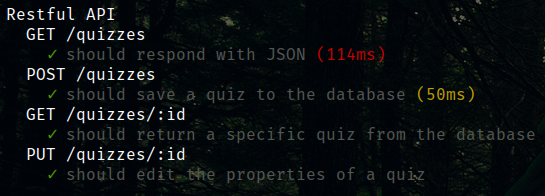
\includegraphics[scale=0.55]{testing/api/api}
  \caption{Test outcome for api.spec.js 1}
\end{figure}
% subsubsection api_spec_js (end)

As can be seen by the little green ticks, all the different HTTP methods passed, proving that the API is working correctly, and thereby allowing requests to be sent from throughout the application. \textit{Success.}



% part testing_ (end)

\section{Acceptance Testing}
The system was passed to a friend for testing, with the request that he note down sections that he both liked and disliked. He had the following positive comments about the application:

\begin{itemize}
  \item The different colour schemes are effective, and are a useful differentiator between the houses. They also give the program a nice, fun feel, which fits in with the audience.

  \item It's very easy to make a quiz, as all the buttons are clear, with all the functions labelled. I think it would be suitable for someone who isn't very skilled with technology.

  \item I really like the bouncing animation on the login screen.

  \item The timer in the play quiz screen makes it really exciting to play on; there's a lot of tension.
\end{itemize}

He also had the following, less positive, notes:

\begin{itemize}
  \item At first I didn't know how to change the question title. You could make this a bit clearer by adding a box around it, or something.

  \item When there are a lot of people on the quiz, the program slows down quite a lot, and the timer bar is very jittery.

  \item It's a shame that there aren't any live visualisations to see what other people are answering.
\end{itemize}

As can be gleaned from the notes above, the tester's overall opinion of the system was strong, especially in the quiz creator interface. This is not surprising, as a large amount of time was spent making this work properly. The quiz playing interface lacks the same amount of polish, and this was picked up by the tester, though he did comment that it was sufficiently tence and exciting due to the inclusion of the live countdown timer.

